\documentclass[dvipdfmx]{jsarticle}
\usepackage{subfigure}
\usepackage{graphicx}
\usepackage{listings,jvlisting}
\usepackage{multicol}
\usepackage{float}
\usepackage{circuitikz}
\usepackage{tikz}
\usepackage{amssymb}
\usepackage{arydshln}
\usepackage{wrapfig}
\usepackage{url}


\begin{document}
\title{グラフ信号処理 第4回目課題}
\date{}
\author{}
\maketitle

\section{頂点領域の信号}
\begin{figure}[h]
  \centering
  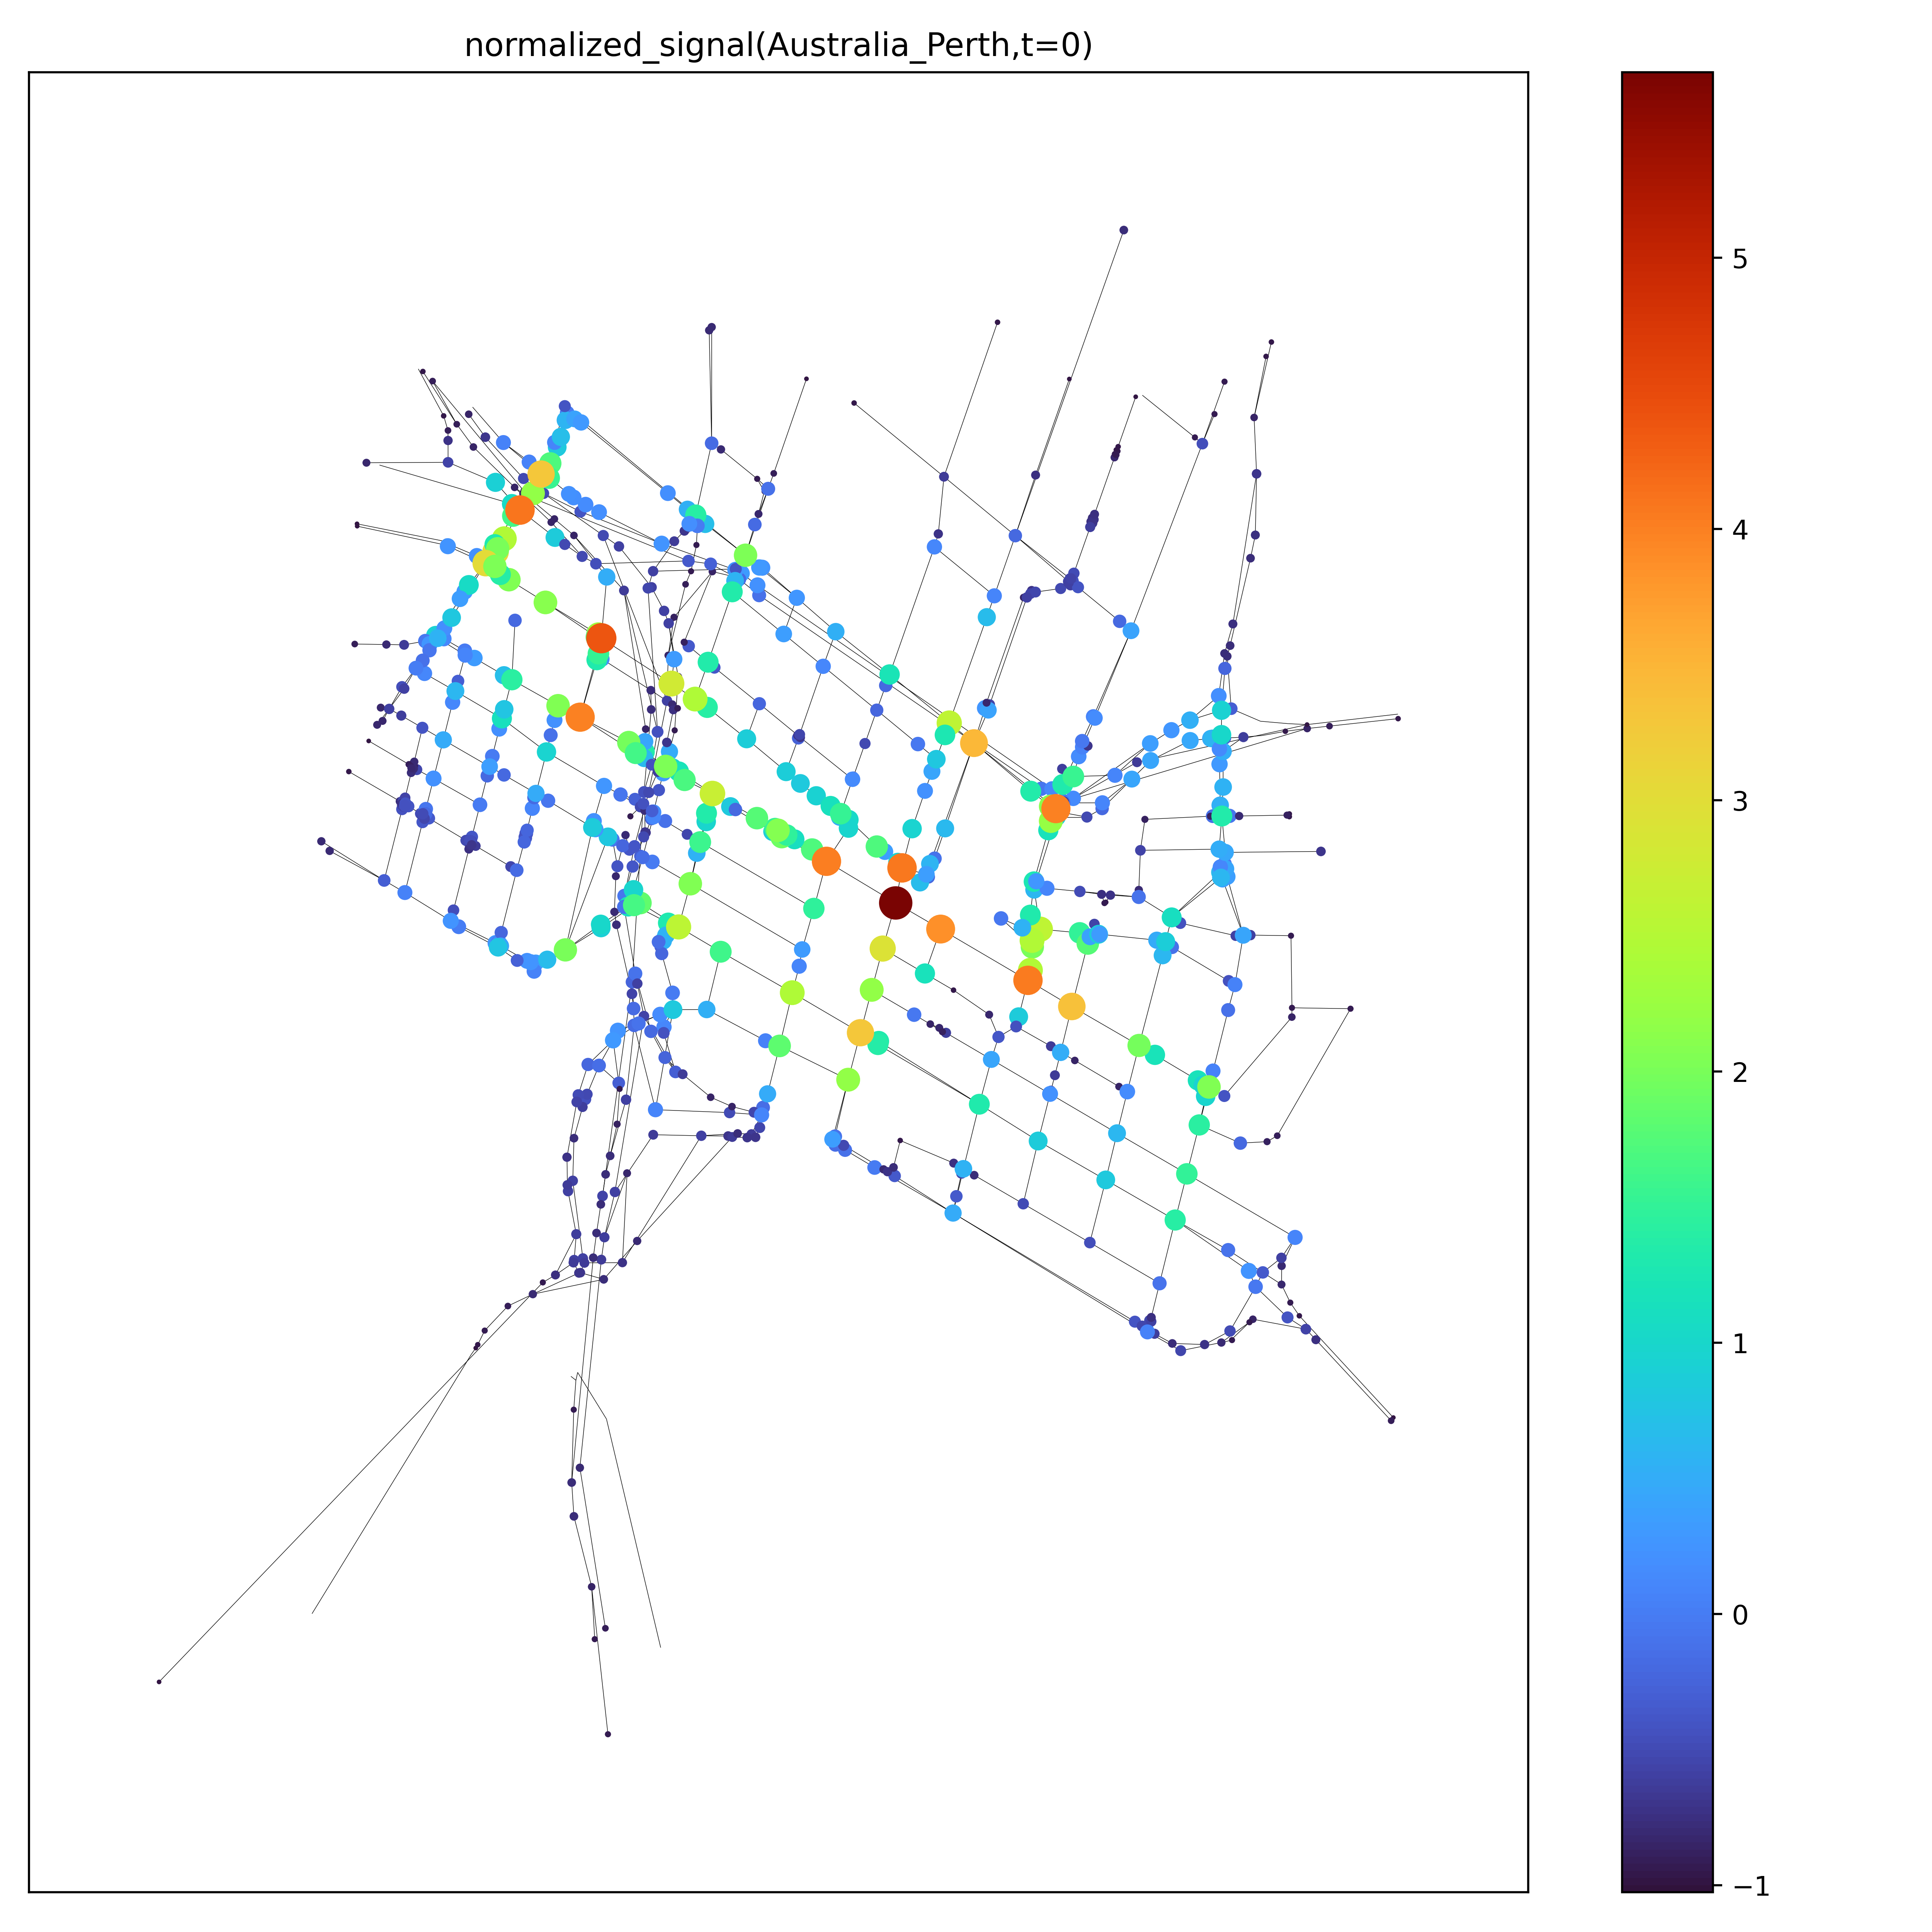
\includegraphics[width=\linewidth]{fig/normalized_signal_Australia_Perth.png}
  % \caption{}
  % \label{fig:}
\end{figure}

\section{グラフフーリエ変換のスペクトル}

\begin{figure}[h]
  \centering
  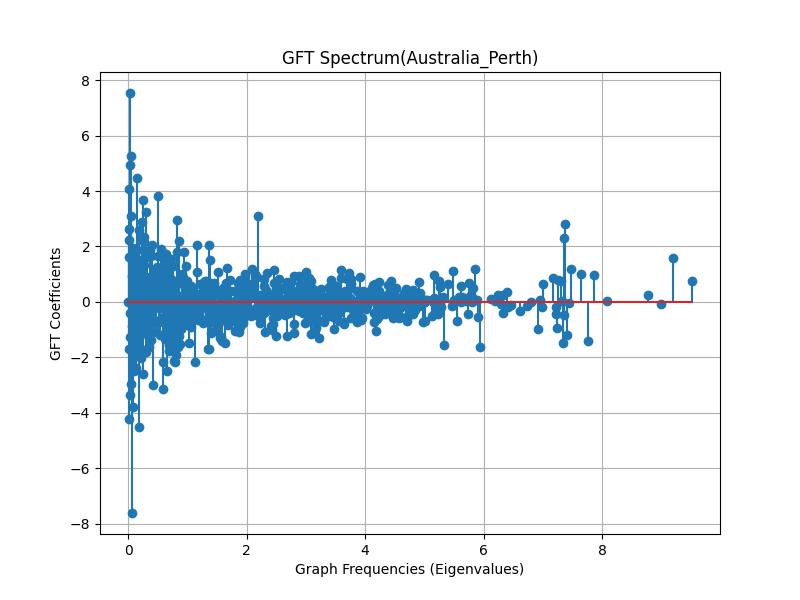
\includegraphics[width=\linewidth]{fig/gft_spectrum_Australia_Perth_test.png}
  % \caption{}
  % \label{fig:}
\end{figure}

\newpage
\section{固有ベクトル毎の頂点領域のグラフ信号}

\begin{figure}[h]
  \centering
  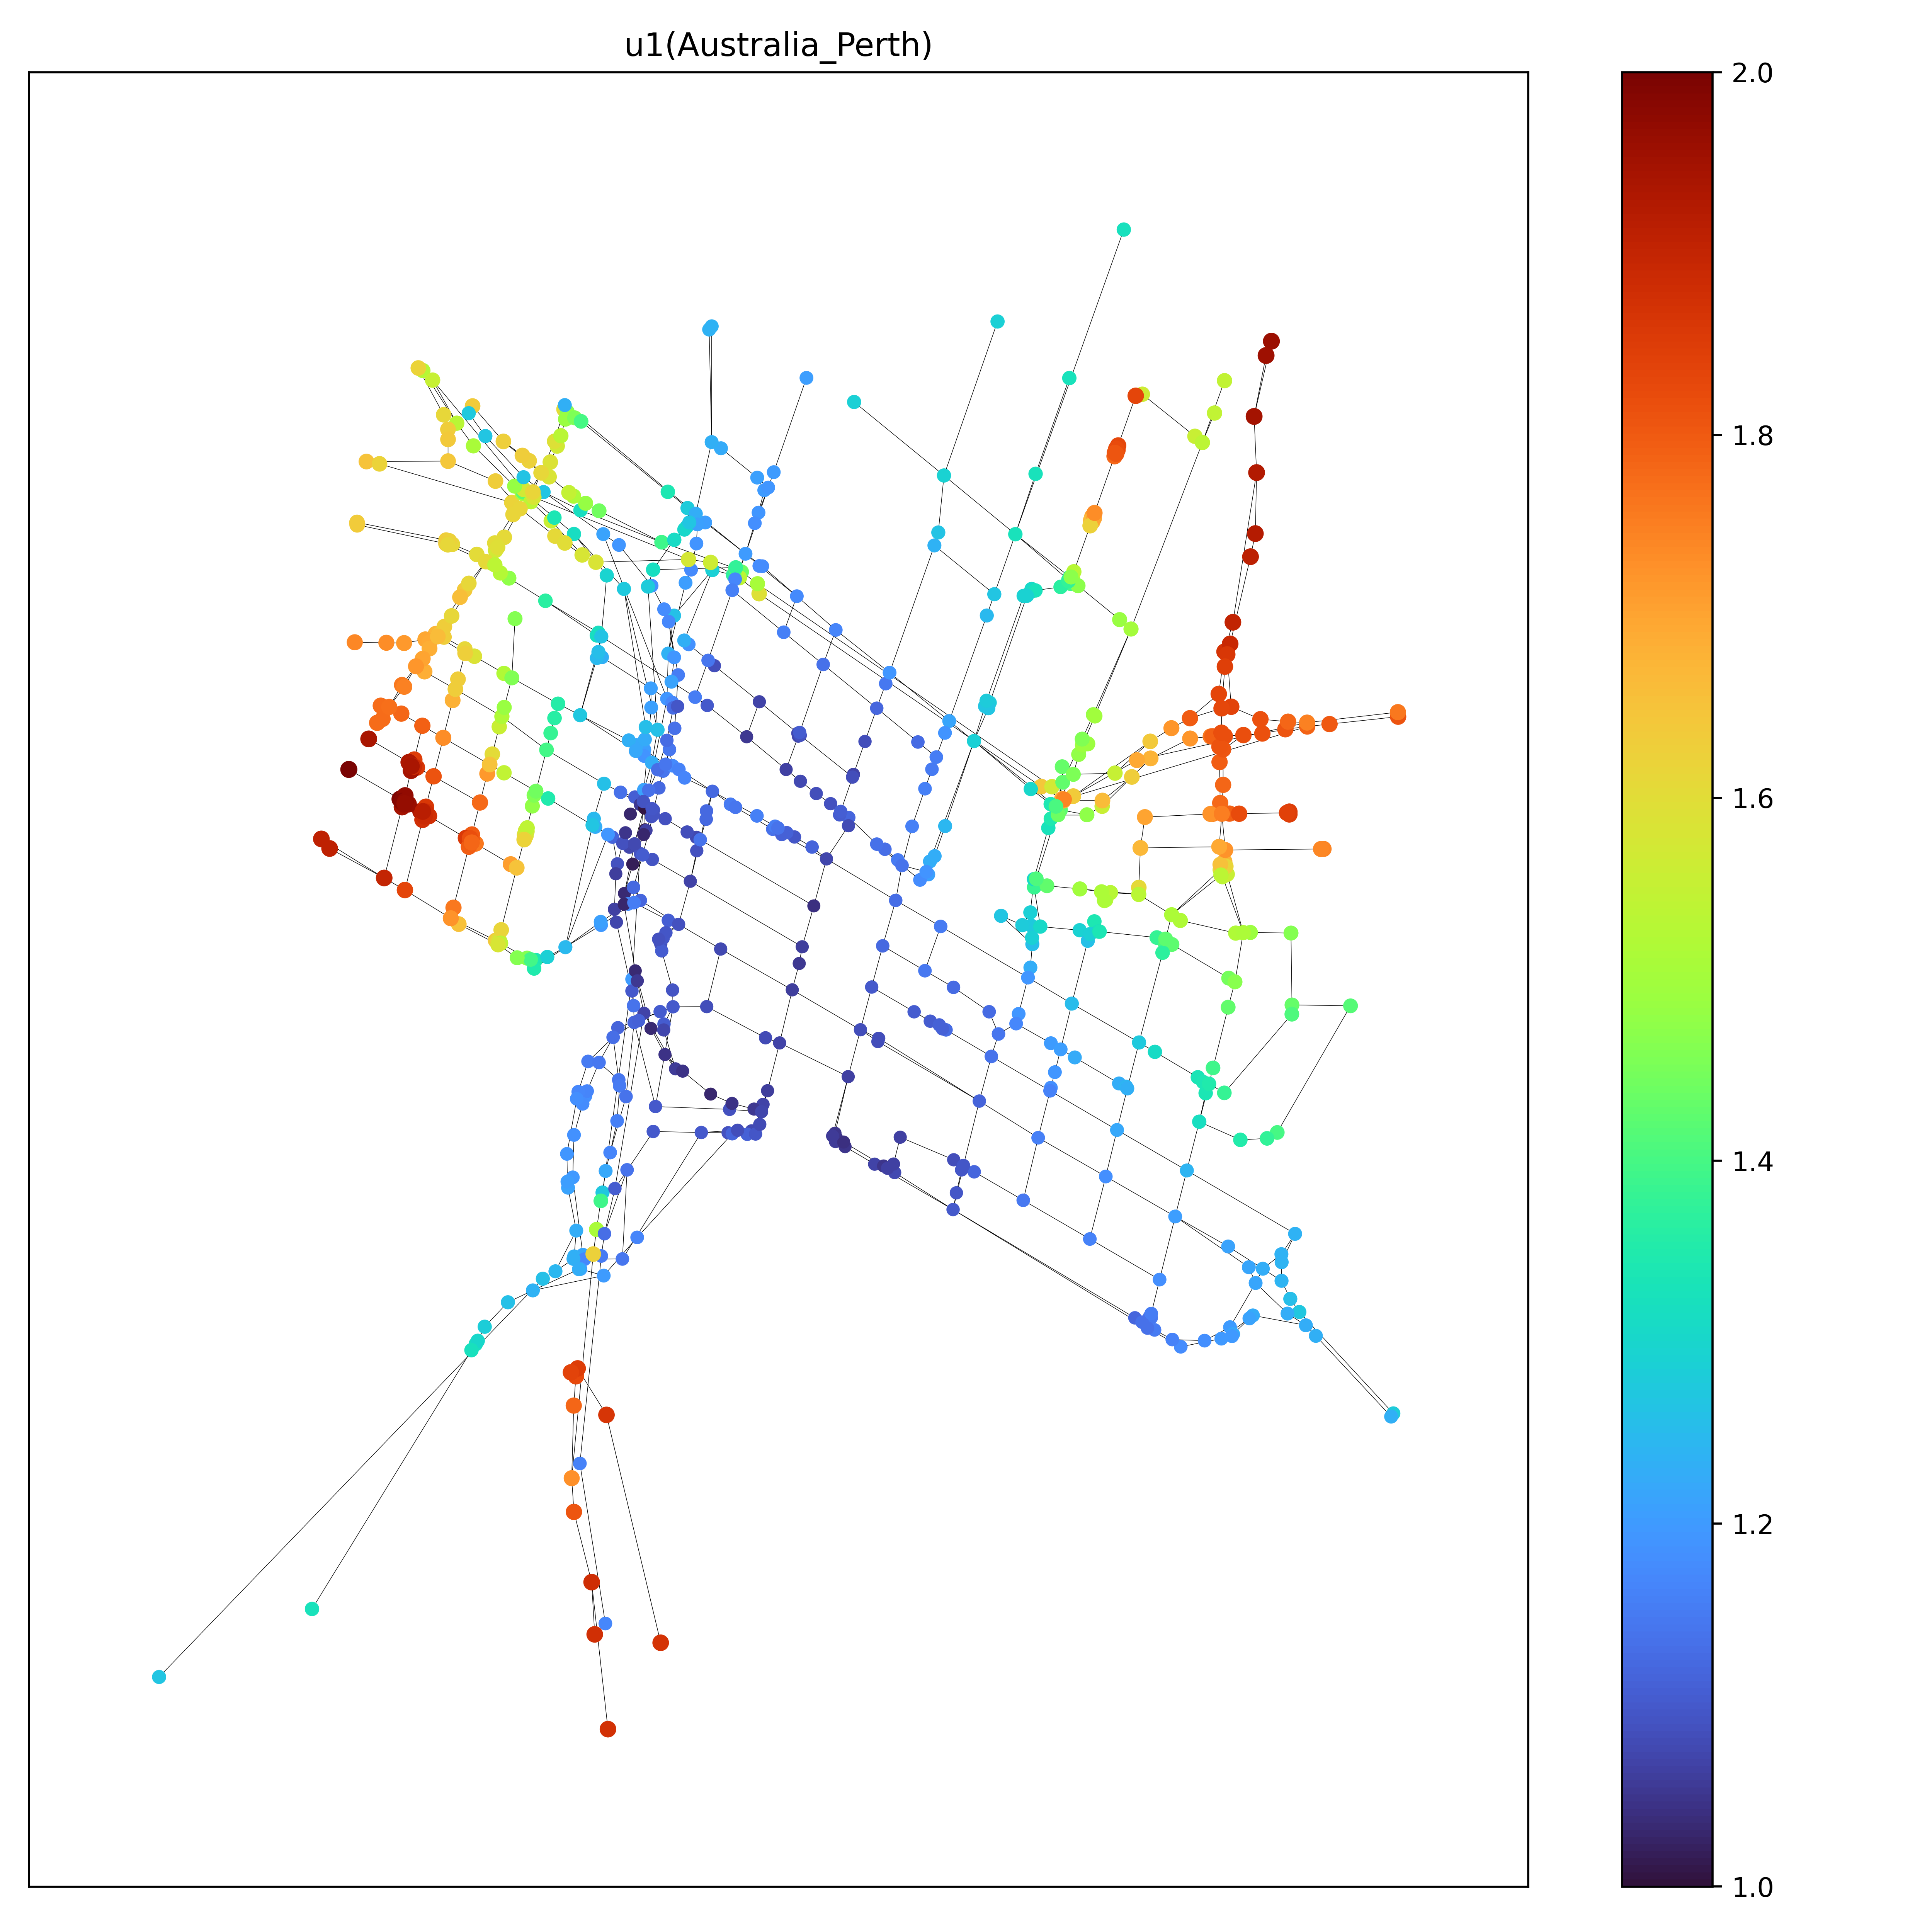
\includegraphics[width=\linewidth]{fig/u1_Australia_Perth.png}
\end{figure}
\begin{figure}[h]
  \centering
  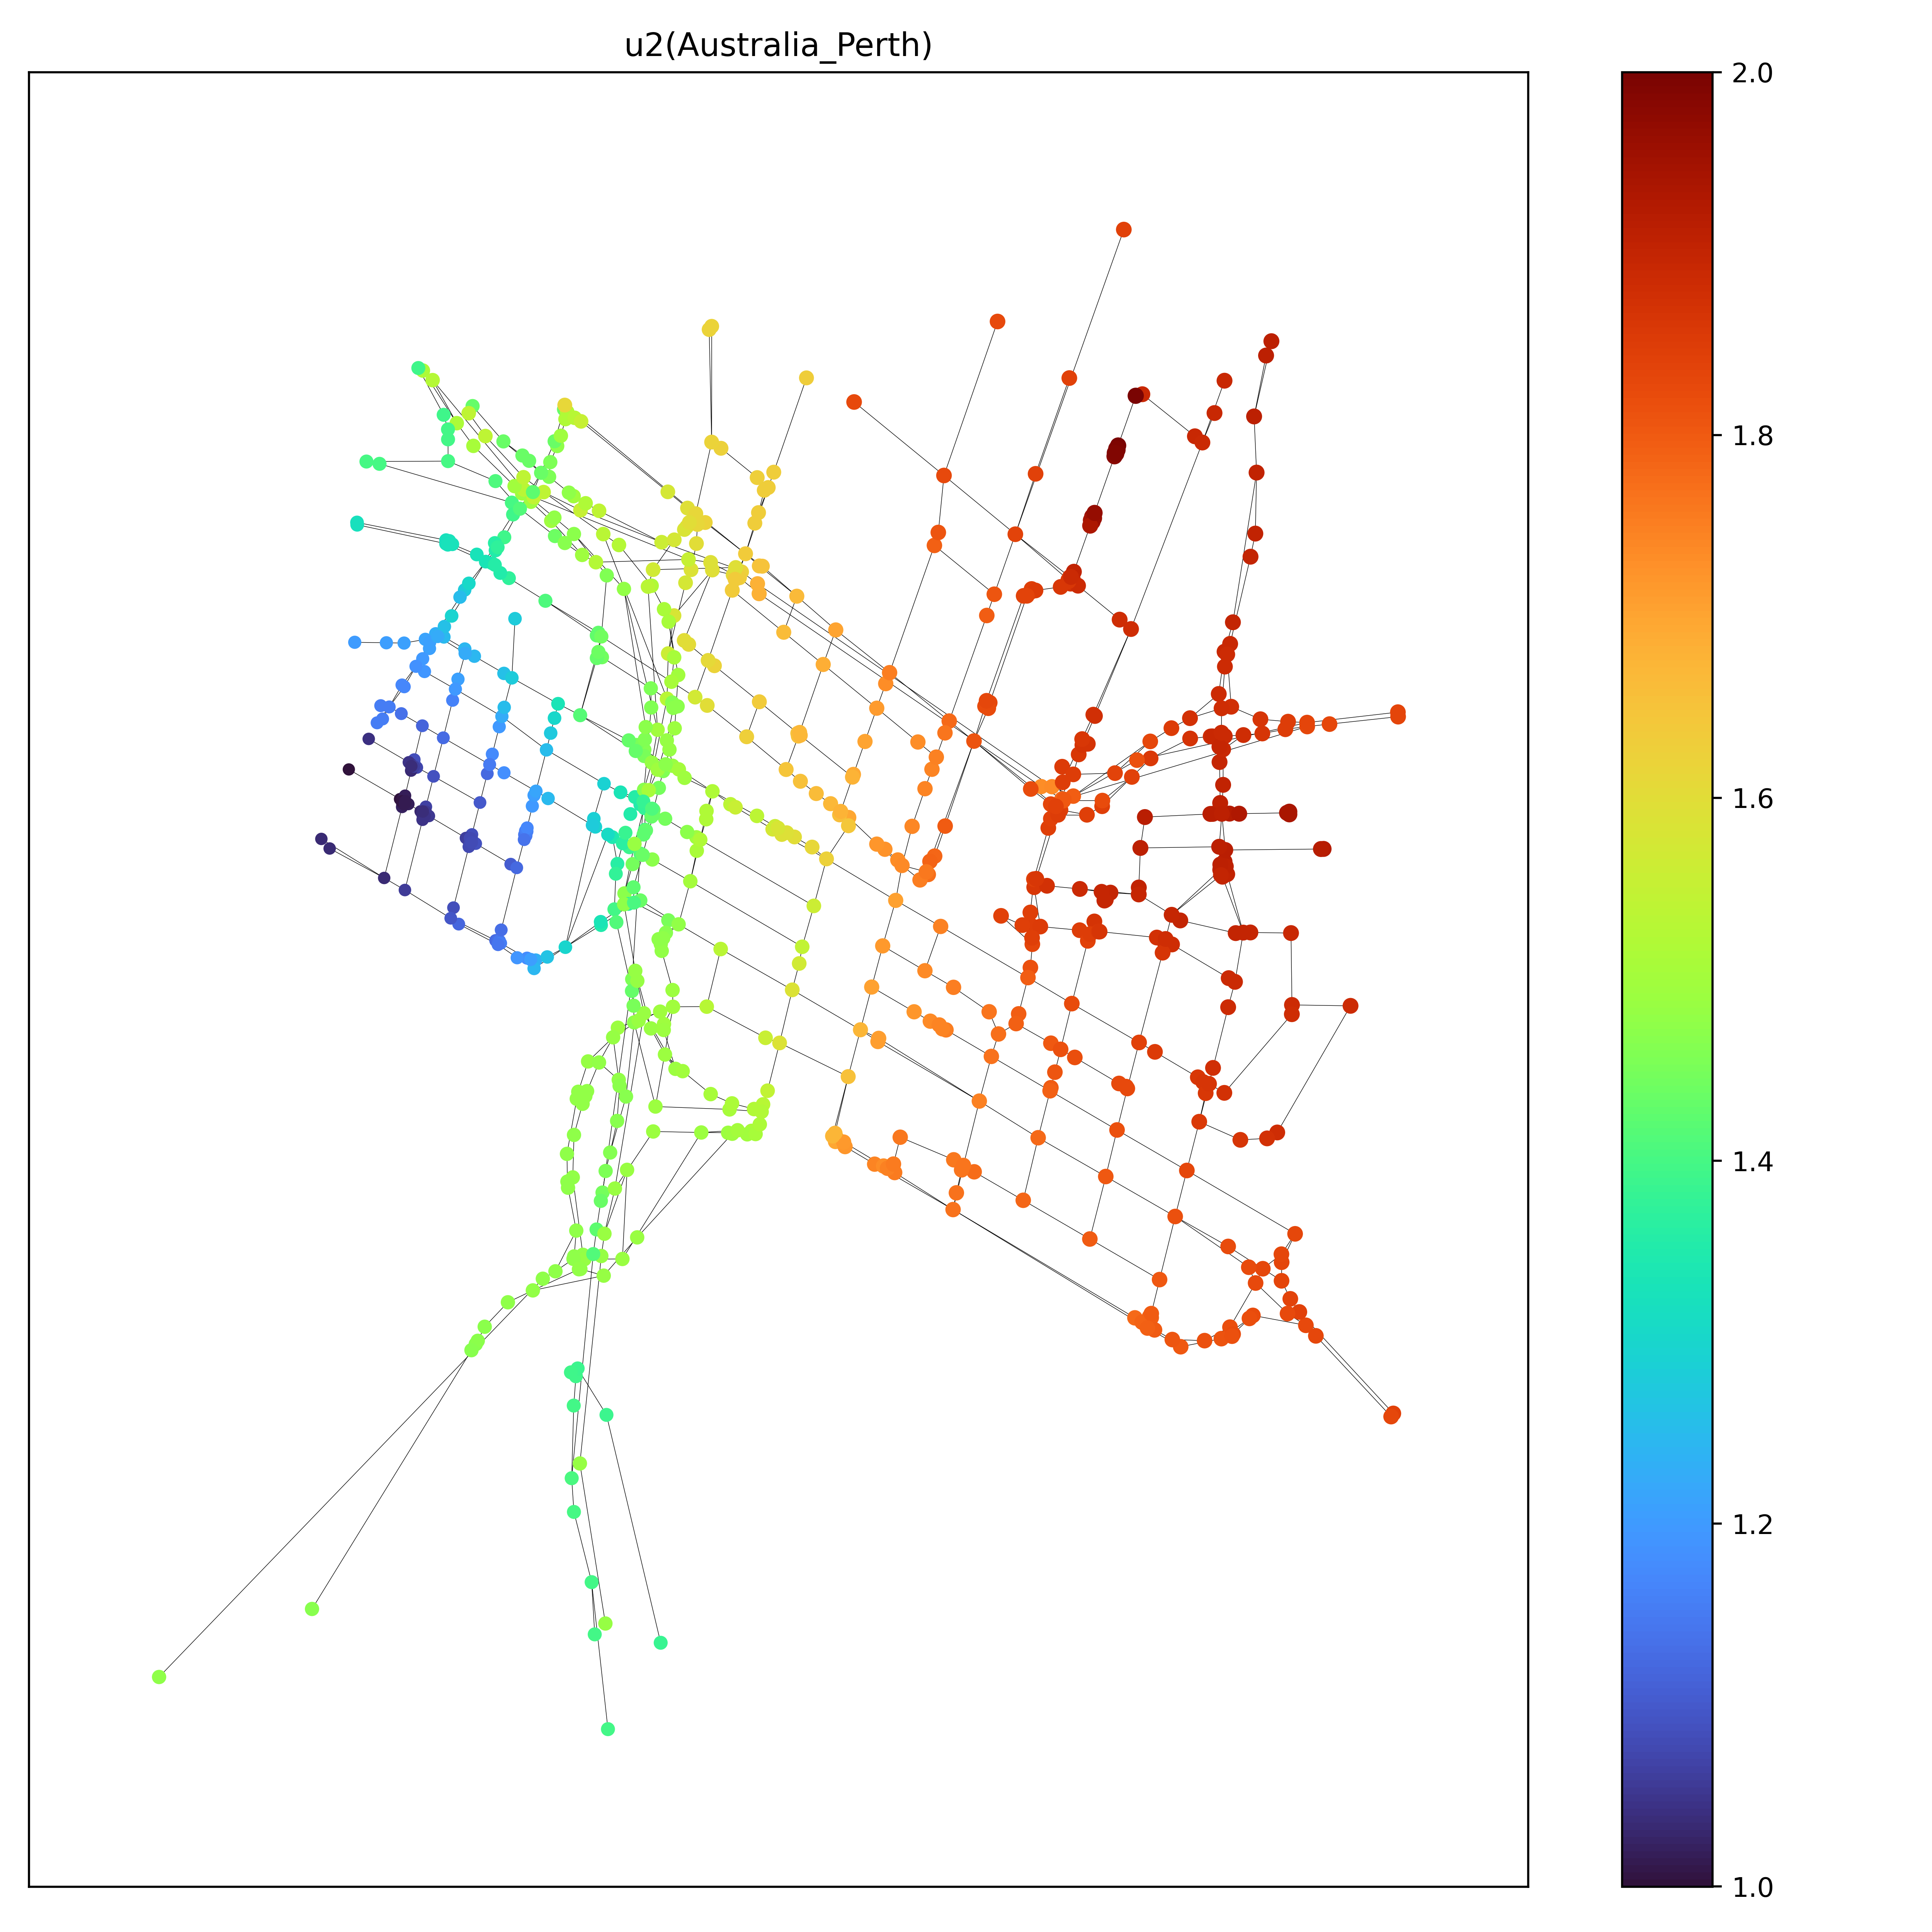
\includegraphics[width=\linewidth]{fig/u2_Australia_Perth.png}
\end{figure}
\begin{figure}[h]
  \centering
  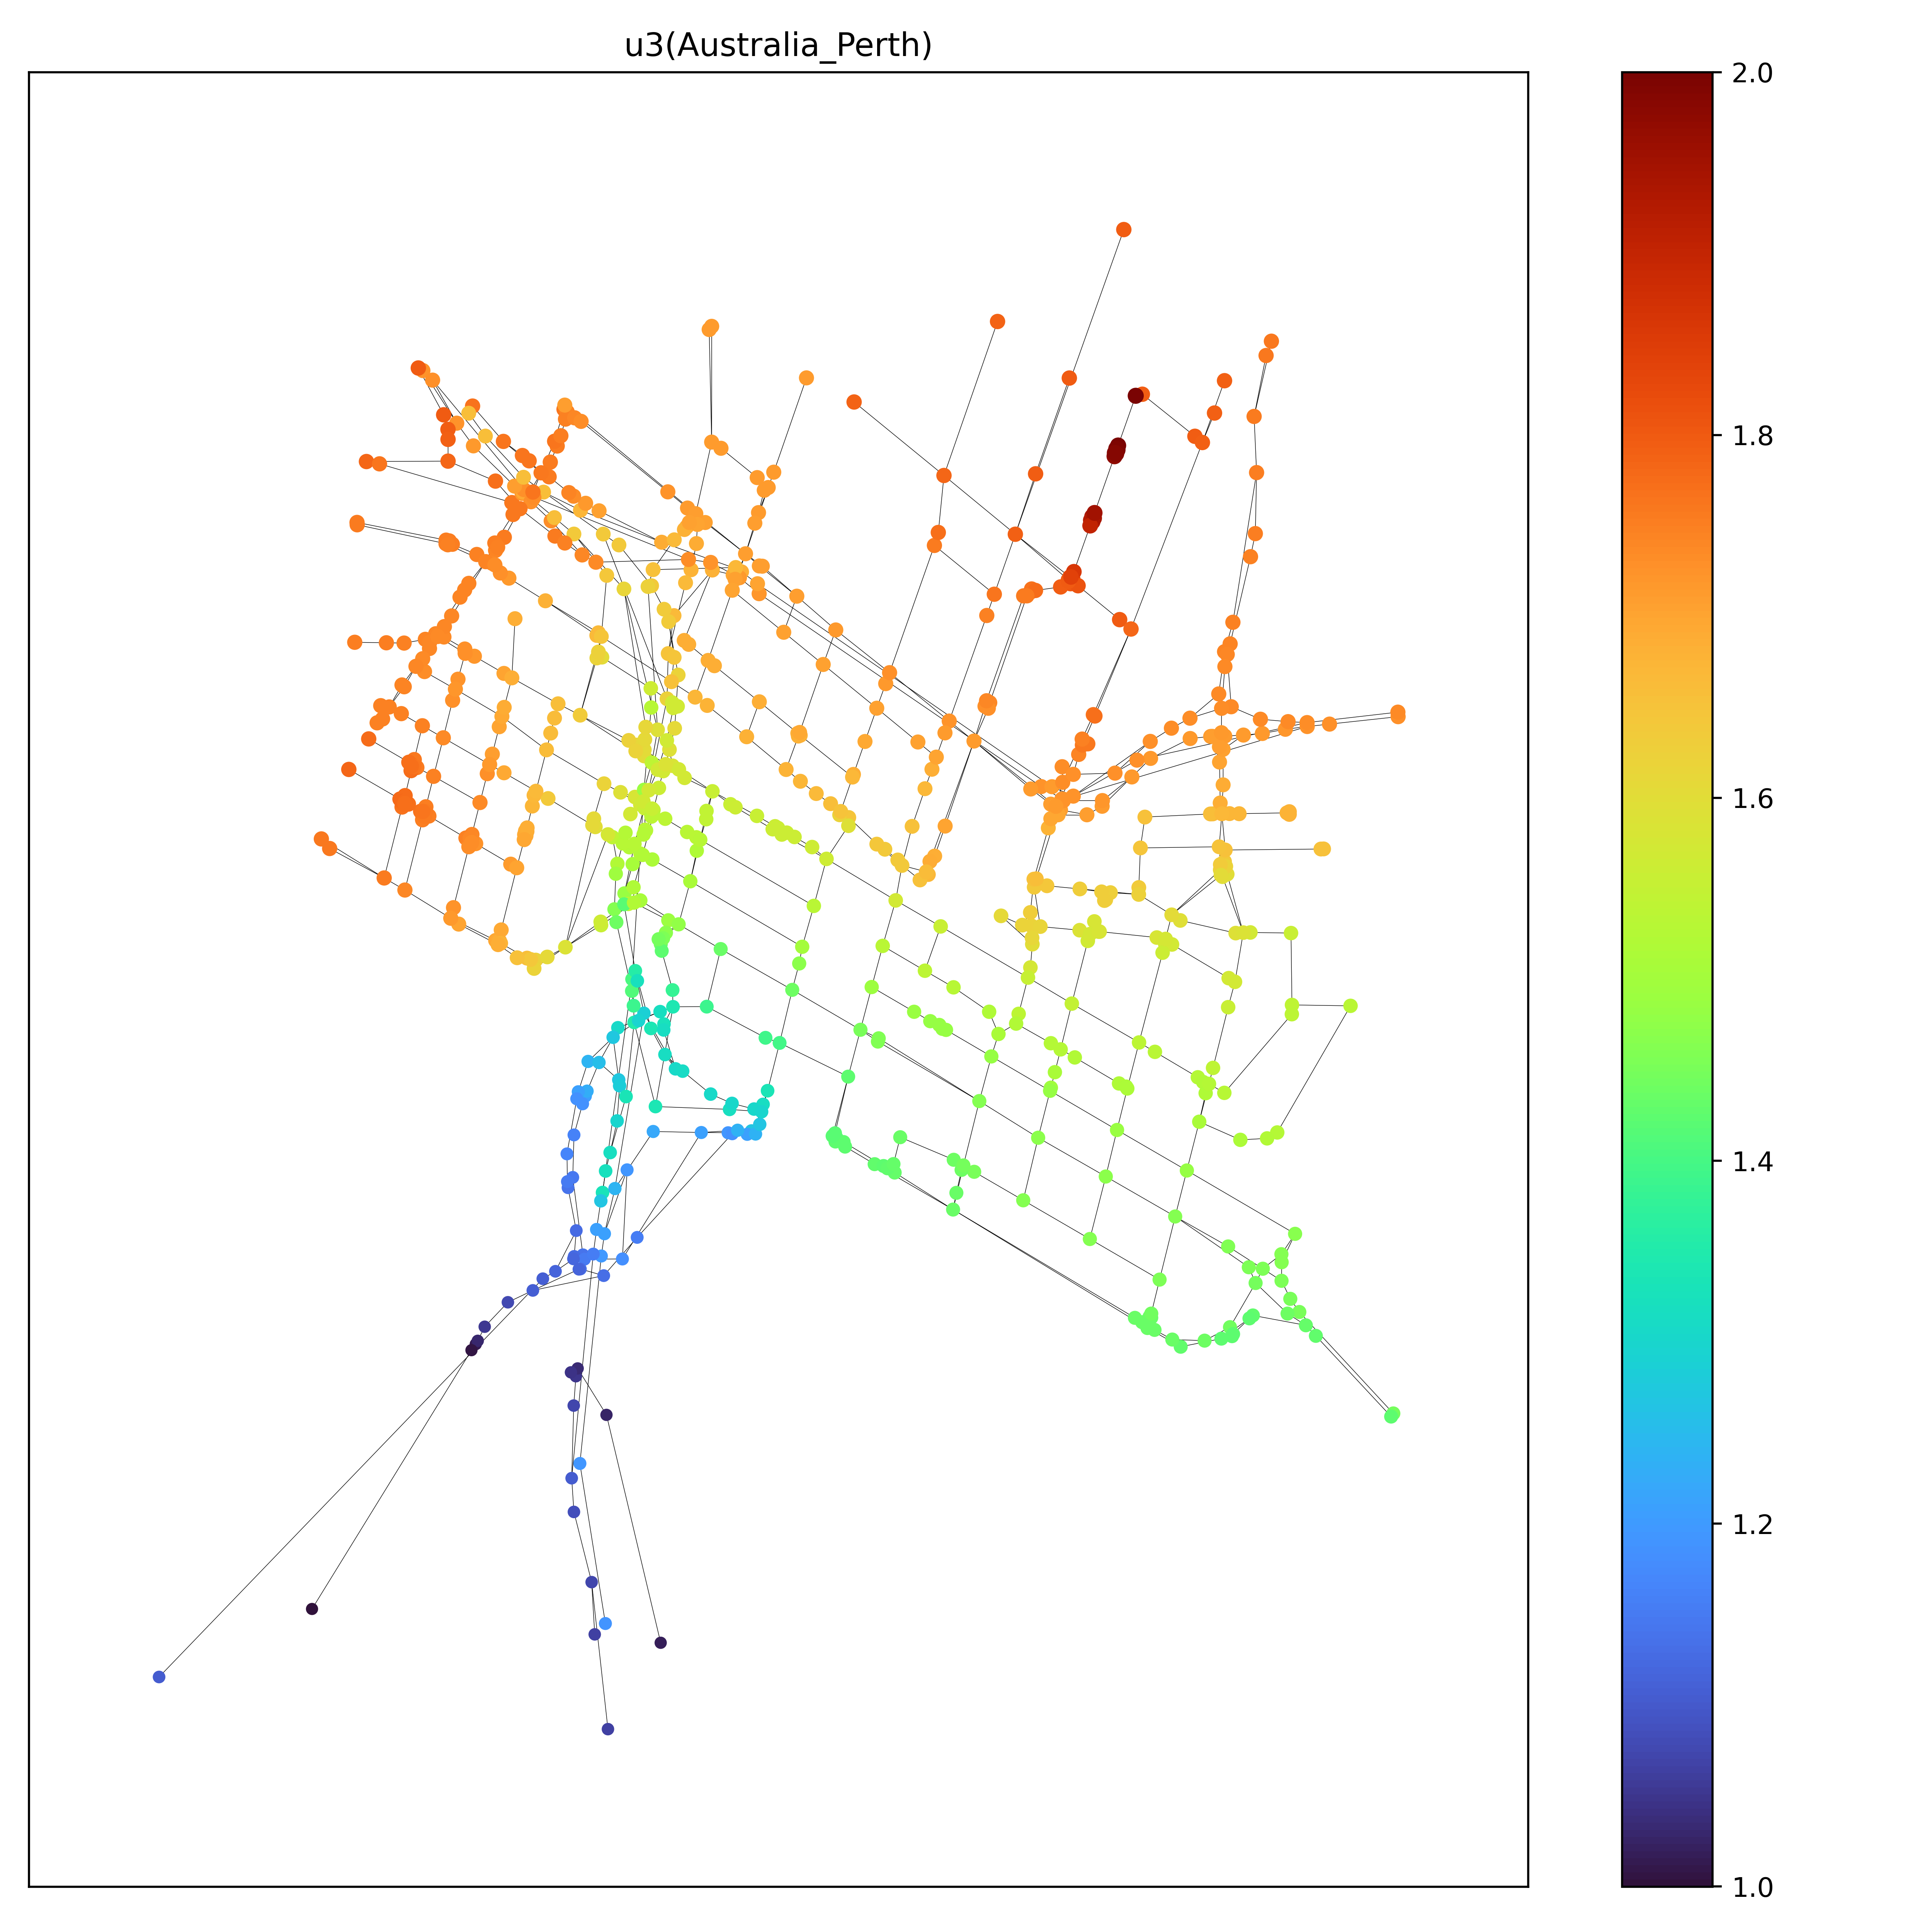
\includegraphics[width=\linewidth]{fig/u3_Australia_Perth.png}
\end{figure}
\begin{figure}[h]
  \centering
  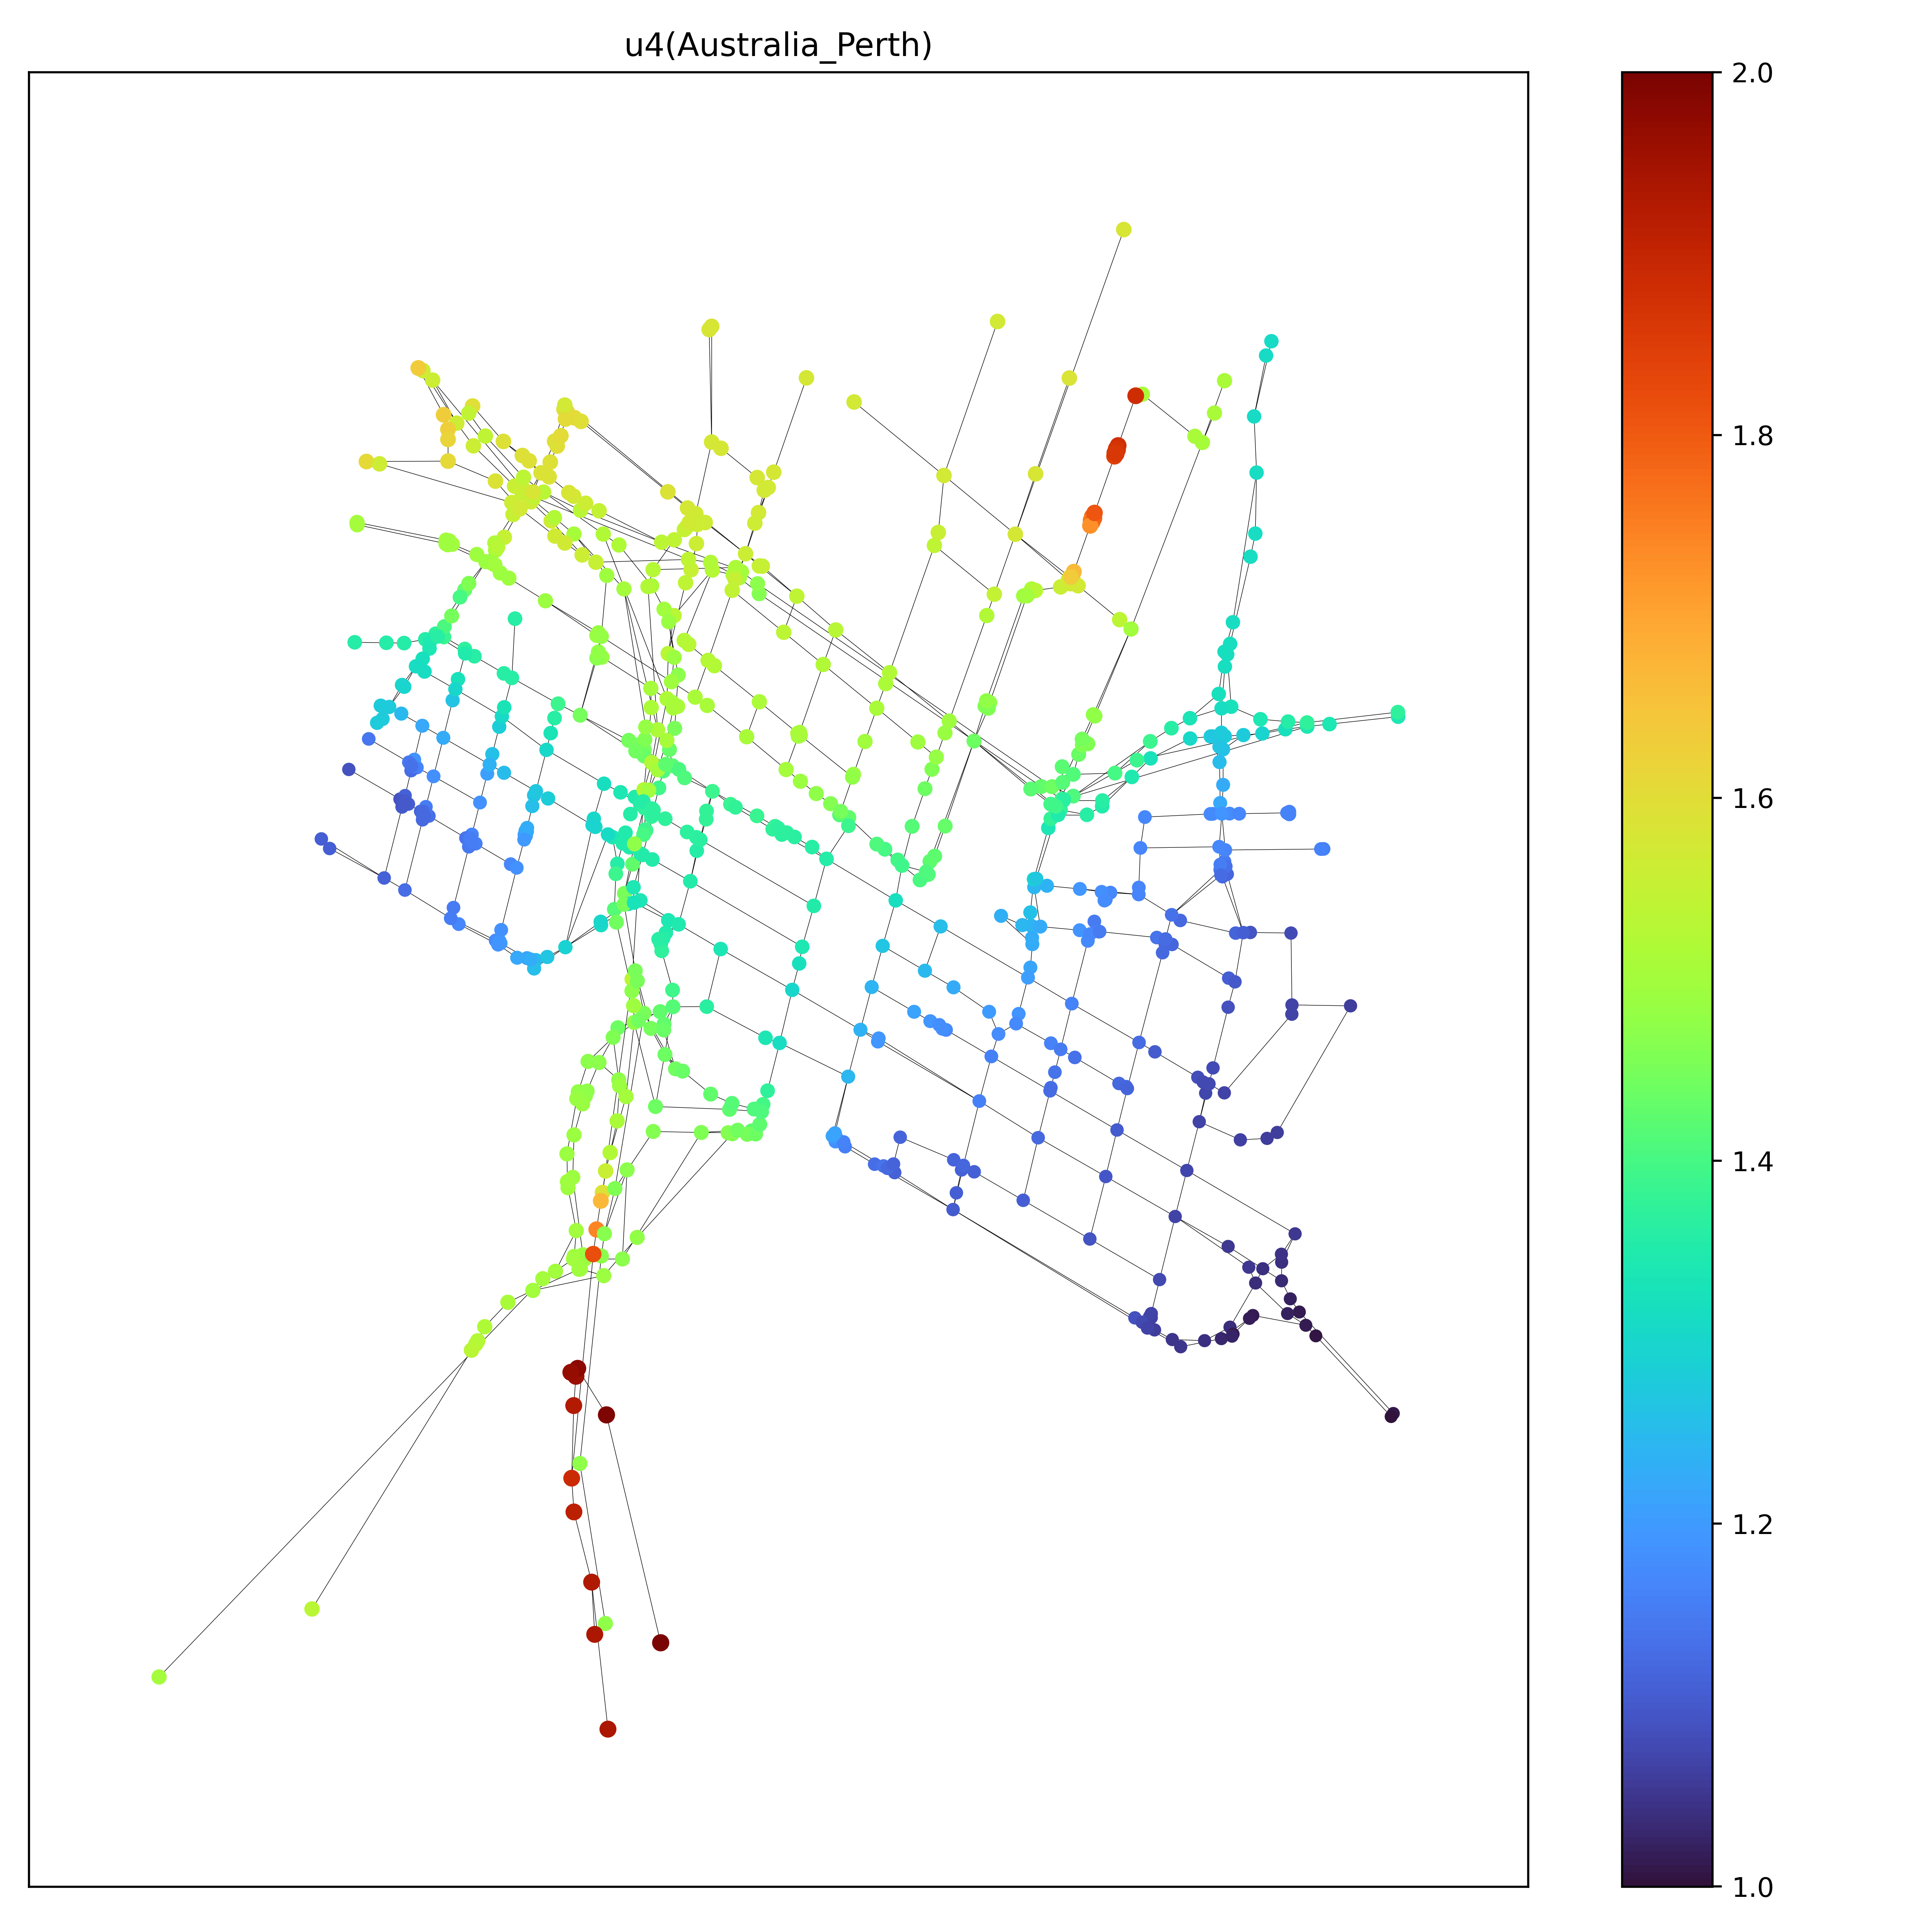
\includegraphics[width=\linewidth]{fig/u4_Australia_Perth.png}
\end{figure}
\begin{figure}[h]
  \centering
  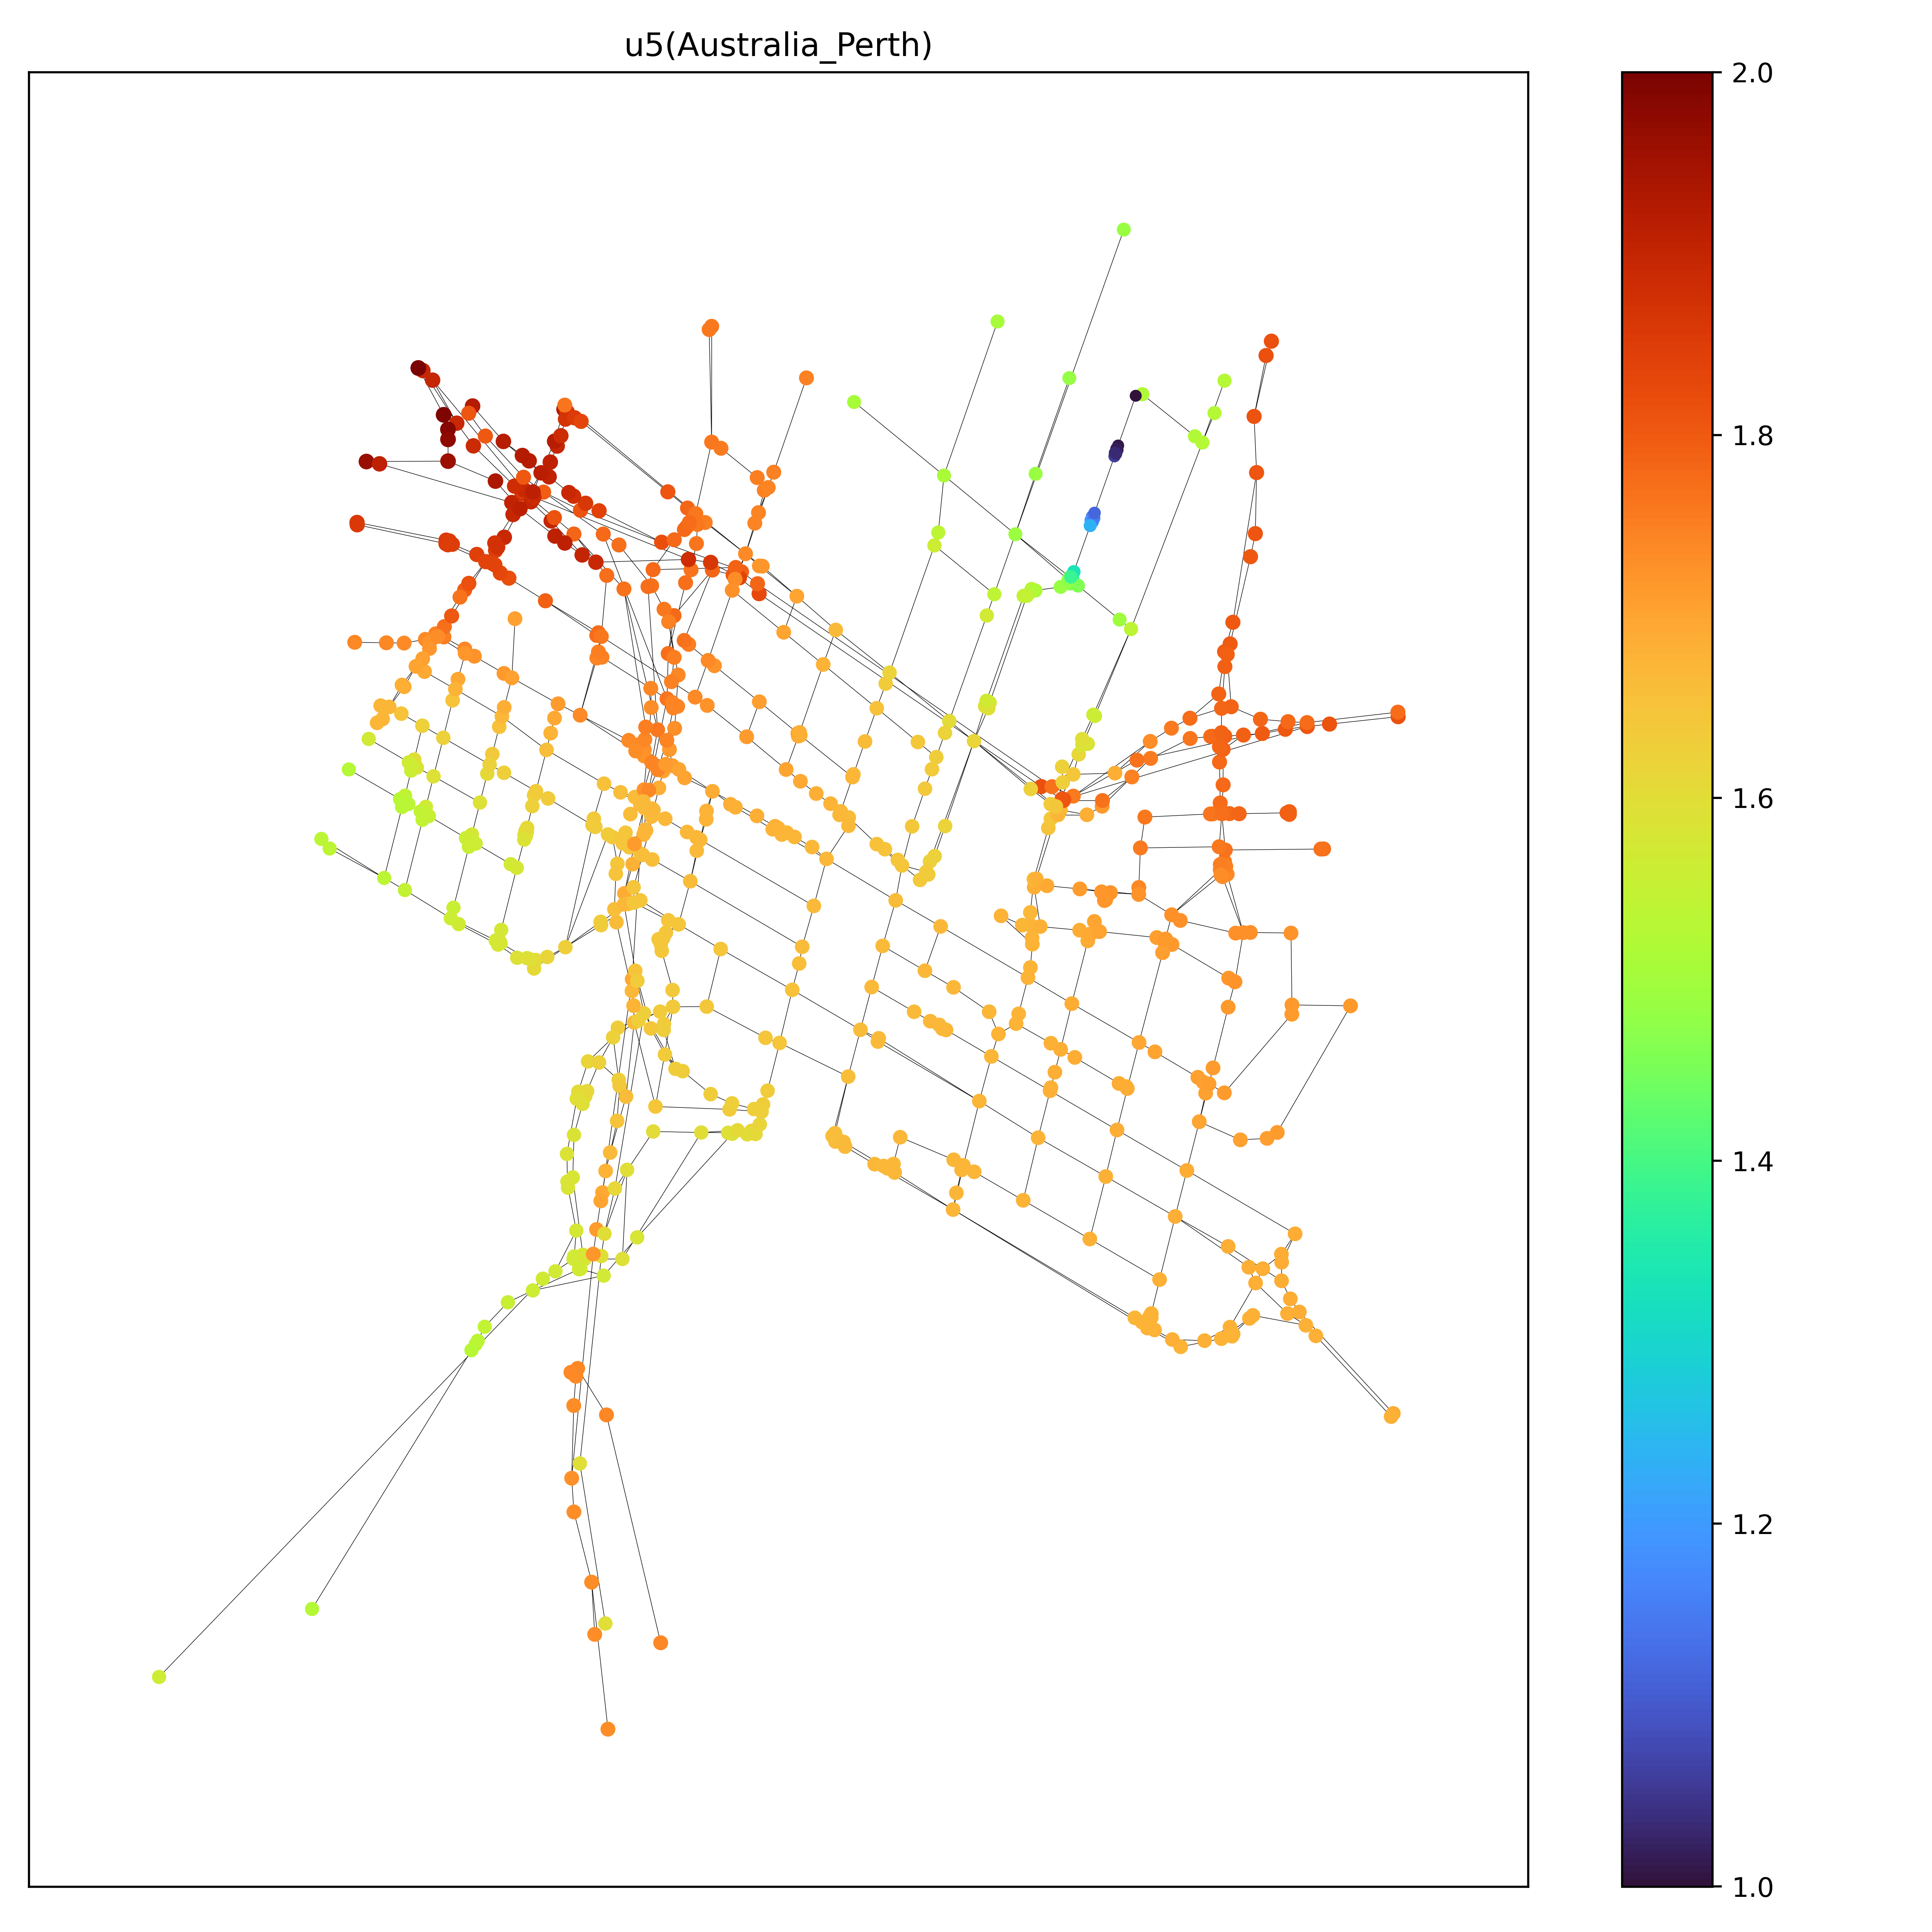
\includegraphics[width=\linewidth]{fig/u5_Australia_Perth.png}
\end{figure}


\end{document}
